\section{Objektorientierung}

\subsection{Klassen und Objekte}{\label{Klassen}}
Klassen bestehen aus \textbf{Variablen} und \textbf{Methoden}.\\
Objekte können aus Klassen erzeugt werden: \verb|Point a = new Point()|\\
Konstruktoren können in den meisten IDEs automatisch generiert werden.

Sofern kein Konstruktor definiert ist, wird der \textbf{Default-Konstruktor} verwendet. Die Instanzvariablen werden mit
Default-Werten initialisiert (primitive mit \verb|0|, Referenzdatentypen mit \verb|NULL|)\\

Klassen arbeiten mit Referenzen, dies muss bei Zuweisungen beachtet werden:
\begin{center}
    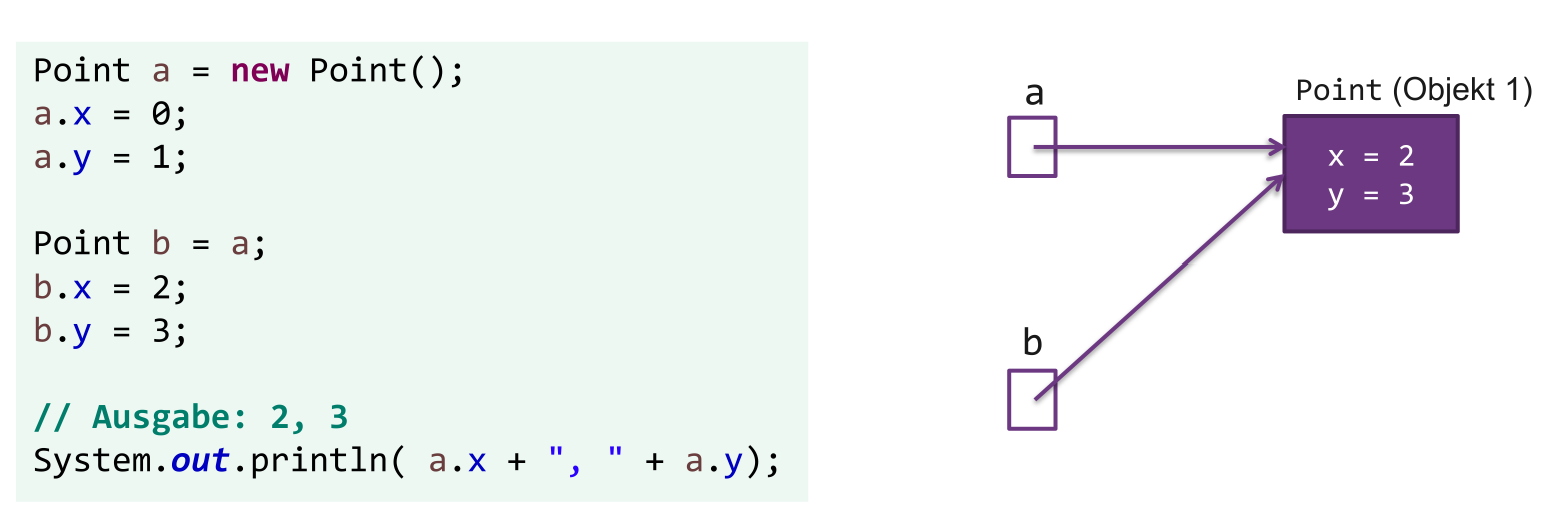
\includegraphics[width=0.9\columnwidth]{pictures/copy-semantics.png}    
\end{center}

\subsection{Methoden}

\subsubsection{Parameter}
Java verwendet \textit{immer} \textbf{Call by Value}. Die Argumente werden kopiert und als Parameter übergeben. Dies kann zu unterschiedlichem Verhalten
je nach Datentyp führen:\\

\textbf{Primitive Datentypen}:\\
Methode arbeitet mit Kopie des Wertes
\begin{center}
    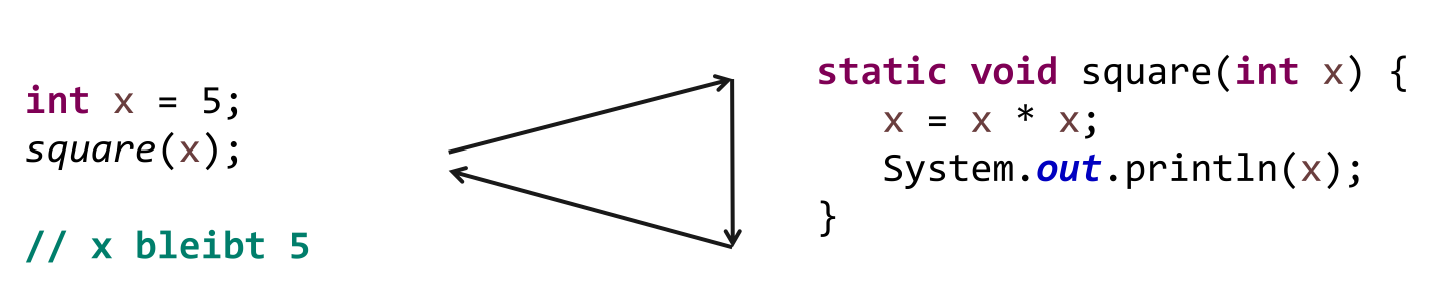
\includegraphics[width=0.9\columnwidth]{pictures/primitive-params.png}    
\end{center}

\textbf{Referenzdatentypen}:\\
Methode arbeitet mit Kopie der Referenz
\begin{center}
    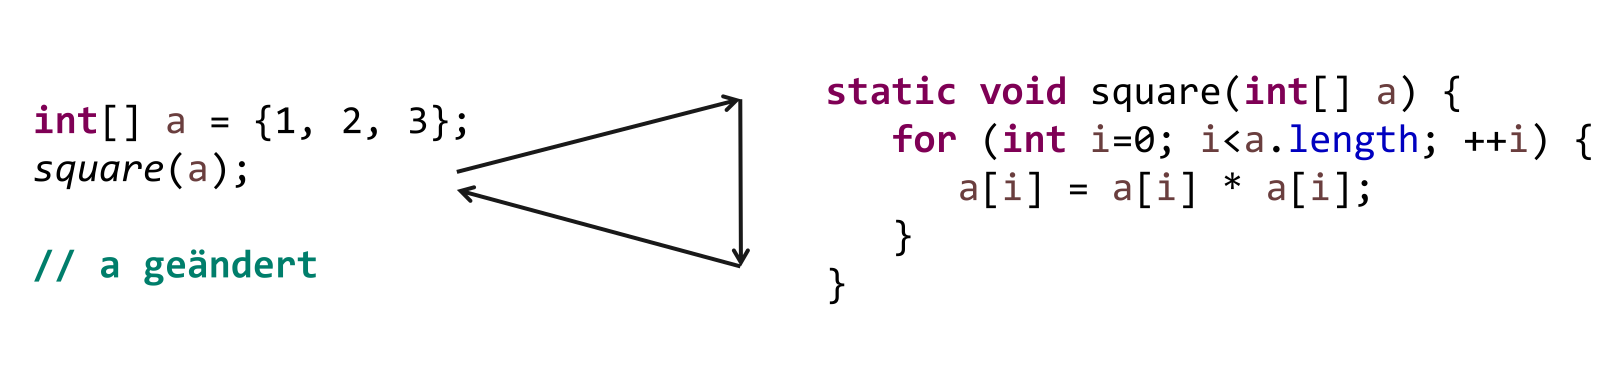
\includegraphics[width=0.9\columnwidth]{pictures/reference-params.png}    
\end{center}

\subsection{Unit Testing}
Unit Testing ist eine der Varianten, um Bugs zu verhindern. In guten Unit Tests sollen möglichst alle relevanten Fälle abgedeckt sein.
Dazu gehören Standardfälle (im Bereich der Funktion) und Edge Cases (z.B. 0, max. und min. Bereich, usw.). Siehe auch \ref{Unit-Test}\\
Faustregel:
\begin{itemize}
    \itemsep0em
    \item Pro Klasse eine Test-Klasse
    \item Pro Testfall eine Methode
\end{itemize}

\subsubsection{Assert-Methoden}
\begin{center}
    \begin{tabular}{ll}
        \rowcolor[RGB]{239,239,239} 
        \textbf{Methode} & \textbf{Bedingung} \\ \hline
        assertEquals(expected, actual) & für prim. und Referenztypen \\
        assertNotEquals(expected, actual) & \\
        assertSame(expected, actual) & actual == expected\\
        assertNotSame(expected, actual) & actual != expected\\
        assertTrue(condition) & condition\\
        assertFalse(condition) & !condition\\
        assertNull(value) & value == null\\
        assertNotNull(value) & value != null\\
    \end{tabular}
\end{center}

\begin{center}
    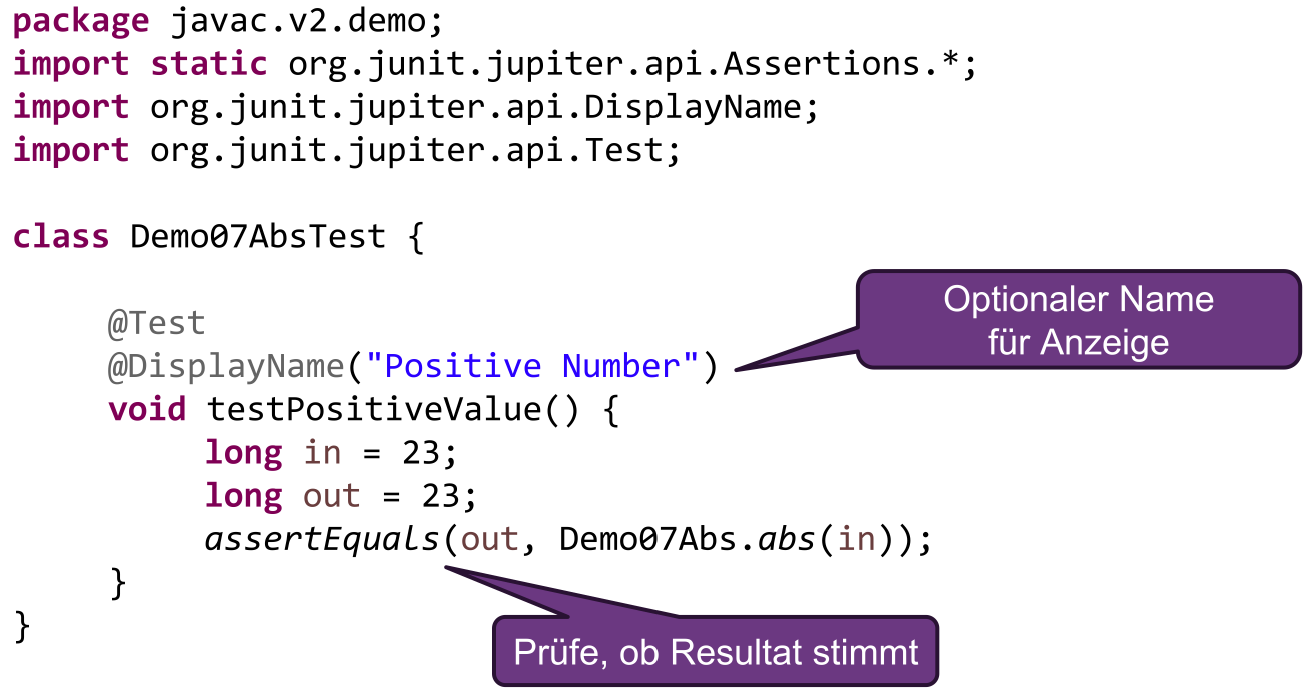
\includegraphics[width=0.9\columnwidth]{pictures/testmethode.png}    
\end{center}

\subsubsection{Sichtbarkeit}
\begin{center}
    \begin{tabular}{ll}
        \rowcolor[RGB]{239,239,239} 
        \textbf{Keyword} & \textbf{Sichtbar für} \\ \hline
        public & Alle Klassen \\
        protected & Klassen im selben Package und abg. Klassen\\
        (keines) & Klassen im selben Package \\
        private & Nur eigene Klasse \\
    \end{tabular}
\end{center}

Für Zugriffe auf \verb|private|-Variablen können Getter- und Setter-Methoden definiert werden. Siehe auch \ref{GetSet}


